\documentclass[11pt, a4paper, titlepage]{article}
\usepackage[margin=3.5cm]{geometry}
\usepackage{graphicx}
\usepackage{xcolor}
\usepackage{minted}

\usepackage[utf8]{inputenc}
\usepackage[english]{babel}
\usepackage[style=ieee, block=ragged]{biblatex}


\begin{document}
\begin{titlepage}
	% Logo at the top within the margins
	\noindent
	
\includegraphics[width=0.15\paperwidth]{logo-mg.png} % Adjust the size as needed
	
	% Title and subtitle with left offset
	\vspace*{0.5\paperwidth} % Adjust the vertical space as needed
	\noindent\hspace*{0.15\paperwidth} % Offset from the left
	\begin{minipage}{\textwidth}
		
		\color[HTML]{0b5394}\Huge Magisim\\
		\color{black}\Large Open source resource center for simulations \\
	\end{minipage}
	
	\vfill % Push the authorship information to the bottom of the page
	\noindent
	\begin{minipage}{\textwidth}
		\normalsize % 12pt font size
		Jonas Cronholm \\
		\textbf{Gymnasiearbete 100 poäng} \\
		\textbf{Klass:} 21 TE \\
		\textit{Teknikprogrammet} \\
		\textbf{Läsåret:} 2023-2024 \\
		\textbf{Handledare:} Peter Eriksson
	\end{minipage}
\end{titlepage}

% Titlepage for arXiv - Needs style changes soon!
% 
%\begin{titlepage}
%	\title{
\includegraphics[width=0.35\textwidth]{magisim_logo256.png}\par\vspace{1cm}Magisim: Open source resource center for electromagnetic simulations \let\thefootnote\relax\footnotetext{Gymnasiearbete 100p}}
%	\author{Jonas Cronholm, Rasmus C. Ljung}
%	\maketitle
%\end{titlepage}
%
\newpage
\
\newpage

\begin{abstract}
	
	With serious competition in the modern market it is not trivial to create a product that can match the expectations of professional users and still appeal to hobby engineers, especially at a modest price point. The gap in capabilities between enterprise and open source simulation software is growing bigger due to lack of funding, which often results in limited research and development for free and open source projects. This growing disparity poses a significant challenge for developers aiming to balance advanced features with affordability. 
	
	Enterprise simulation software benefits from substantial financial backing, enabling teams to invest in cutting-edge research, continuous enhancements, and dedicated customer support. This translates to robust features, high accuracy, and comprehensive technical support, making them the preferred choice for intricate and mission-critical projects. However, the cost associated with these solutions can be prohibitive for smaller businesses and individual hobbyists. This gap is further exacerbated by the intricate nature of simulation software. Meeting the needs of professionals frequently involves complex algorithms, intricate modeling, and high-performance computing. Striving to offer similar capabilities within a modest price range for hobbyists can be daunting, as the associated costs can quickly spiral upwards.
	
	Addressing this challenge, Magisim, an open-source project, is introduced as a versatile solution, leveraging parallelization to enhance simulation efficiency and accessibility. Designed primarily as an educational tool, Magisim integrates a wide range of simulation algorithms with a node graph interface, simplifying the dataflow programming for users of varying expertise. The cornerstone of Magisim's innovation lies in its implementation of parallel computing techniques. By harnessing the power of parallelization, Magisim significantly reduces computational time and resource requirements, making advanced simulations more accessible to amateurs and cost-effective for professionals. This approach not only democratizes the learning and application of complex simulations but also bridges the gap in performance between high-cost enterprise solutions and open-source software. Consequently, Magisim serves as a testament to the potential of open-source development in narrowing the divide in technological capabilities, fostering an environment where both professionals and hobbyists can explore, learn, and contribute to the evolving field of simulation and data analysis.
	
	
	%This paper presents a proof-of-concept software project that aims to illustrate the potential of open source magnetic field simulations utilizing parallelized computing techniques on consumer-grade hardware. Magnetic field simulations hold immense significance across scientific, engineering, and technological domains, yet their resource-intensive nature often limits accessibility, particularly in the context of proprietary software and high-cost hardware. By conducting a thorough analysis of existing open source simulation tools, parallel computing frameworks, and optimization strategies, we lay the groundwork for a proof-of-concept that showcases the potential of democratizing magnetic field simulations. This paper provides an in-depth exposition of the technical underpinnings involved in parallelization implementation, optimization techniques, and comprehensive performance evaluations. Through our preliminary experimentation, we offer empirical evidence of substantial reductions in simulation runtime while maintaining accuracy levels comparable to established proprietary solutions.
	
	%Moreover, the paper acknowledges and addresses the inherent challenges intrinsic to parallel programming, hardware limitations, and scalability concerns when deploying simulations on consumer-grade hardware. By providing practical insights and strategic recommendations, we outline potential avenues to navigate these challenges and attain optimal performance across varying hardware configurations.
	\begin{flushleft}
		{\small {\bf Keywords:} Computational electromagnetics, CEM, MoM, FEM, parallelization, simulator, CUDA, gradio, Data Analysis, Visualization}
	\end{flushleft}
	
\end{abstract}
\refstepcounter{page}
\setcounter{page}{2}
\tableofcontents
\newpage
%\twocolumn[]
\section{Introduction}
\subsection{Background}
The field of radio engineering, particularly within the amateur radio sphere, necessitates a deep understanding of electromagnetic (EM) theory and its practical applications. Traditionally, this domain has been supported by a variety of simulation tools, aiming to provide insights into the complex interactions of electromagnetic fields with their surrounding environments. However, a significant challenge has emerged from the existing landscape of these simulation tools, marked by their prohibitive cost and steep learning curves. This divide presents a substantial barrier to entry for amateur radio enthusiasts and learners, who often seek both affordability and simplicity in educational resources. 

\subsection{Problem}
Historically, professional-grade simulation software in electromagnetics has been tailored to meet the demanding needs of industry experts, incorporating advanced features and comprehensive simulation capabilities. While powerful, these tools come at a price point that is often beyond the reach of hobbyists and educational users. Concurrently, the free or low-cost alternatives available in the market tend to compromise either on the width of features or on user accessibility. The complexity of these tools, coupled with often inadequate documentation, further exacerbates the challenge for those new to the field, impeding practical, hands-on learning.

This gap in the market led to the conceptualization of Magisim, initially envisioned as a user-friendly and cost-effective simulator specifically for electromagnetics. Targeted towards the amateur radio community, the primary goal was to demystify EM theory through interactive simulations, making it more approachable for non-professionals. However, as the project progressed, we realized the broader potential for the underlying technology. The modularity of our initial design, made the software applicable in more fields related to simulations or data analysis. This steered the development of Magisim towards becoming a more versatile platform, transcending its original scope.
\newpage

\subsection{Introduction to Computational Electromagnetics}
Computational electromagnetics (CEM) is a field of study that employs numerical methods to solve problems that involve electromagnetic interactions. These computational methods are essential for designing, analyzing, and optimizing electronic and optical devices, such as antennas, radar, waveguides, and optical fibers.

A key technique in CEM is the Finite-Difference Time-Domain (FDTD) method, which simulates electromagnetic field behavior by solving Maxwell's equations across a discretized spatial and temporal grid. This method is prized for its ability to model complex interactions in various materials and structures accurately. FDTD is particularly useful in fields such as antenna design, optical device analysis, and electromagnetic compatibility testing. It allows for a detailed examination of how electromagnetic waves propagate and interact with their environment, making it an essential tool for both researchers and engineers. In educational settings, tools like Magisim utilize FDTD to help students and hobbyists understand and visualize electromagnetic phenomena in a straightforward and accessible manner.


\subsection{Related Work}
\subsubsection{Proprietary Software}
Many solutions exist for simulating electromagnetic systems, particularly in the realm of proprietary software that offers advanced capabilities but often at a cost that is prohibitive for amateurs. Tools like Ansys HFSS, Altair FEKO, and XFdtd are common in this field, each providing specialized features tailored to complex and precise electromagnetic simulation needs.

\textbf{Ansys HFSS (high-frequency structure simulator)} excels in using the Finite Element Method for detailed electromagnetic field simulations, ideal for high-frequency electronics and antenna design. \textbf{Altair FEldberechnung für Körper mit beliebiger Oberfläche (FEKO)} offers a broad range of computational methods, making it versatile for applications across electromagnetic compatibility and antenna design, amongst others. \textbf{XFdtd} utilizes the Finite-Difference Time-Domain method, suitable for transient electromagnetic simulations and interactions, such as EMC testing and bioelectromagnetic analyses.

Despite their robust features and extensive applications, these tools are often not accessible to the common amateur due to their high cost and the complex technical expertise required. This creates a significant barrier for hobbyists and smaller enterprises who might not have the resources or need for such advanced functionalities.
\newpage

\subsubsection{Open Source Projects}
In the field of electromagnetic simulations, the openEMS tool, described by Liebig et al. (2012), stands out as a noteworthy open-source platform leveraging the Finite-Difference Time-Domain (FDTD) method. This tool, freely available to the public, supports various simulation needs, particularly for high-frequency electromagnetic applications. The openEMS platform uses an equivalent-circuit (EC) FDTD method, which simplifies the implementation of material dispersion, thus enhancing the simulation of complex electromagnetic environments. Although openEMS is a powerful tool, its depth and the required scripting for setup and control can be daunting for amateurs and new users.

In his PhD thesis, Novel architectures for brain-inspired photonic computers. Ghent University (2020), Floris Laporte employs a custom Finite-Difference Time-Domain (FDTD) simulator to analyze photonic structures that mimic neural processes for neuromorphic computing applications. Laporte's work focuses on the simulation aspect, using this method to delve into the dynamic behaviors of photonic cavities and their potential as elements in brain-inspired computing architectures. In developing our simulator, Magisim, we have integrated Laporte's FDTD code as a core component.

\newpage
\subsection{Method}
The initial phase of the project involved comprehensive planning using the Kanban system implemented through Atlassian Trello. This enabled efficient organization and prioritization of envisioned functionalities for the simulator and its interface. The systematic arrangement of tasks on the Kanban board facilitated a clear visualization of the project scope, ensuring effective integration of all functionalities. Subsequently, a Gantt chart was utilized to structure the project's timeline and responsibilities, allowing for a detailed outline of the time plan and division of labor.

\subsubsection{User Interface}

Following the establishment of the project's framework and timeline, focus shifted to the user interface (UI) design for Magisim. Several UI development toolkits, including QT and GTK, were evaluated to determine the most suitable option based on modularity, integration ease, and development efficiency. Despite the robust features of QT and GTK, challenges were encountered with their steep learning curves and complex integration processes, including licensing constraints.

The search ultimately led to the selection of Gradio, a novel UI library distinguished by its modular design and streamlined development process. Gradio's capability for rapid prototyping and its intuitive user experience made it the preferred choice for the project, facilitating the swift iteration of UI components.
\begin{center}
	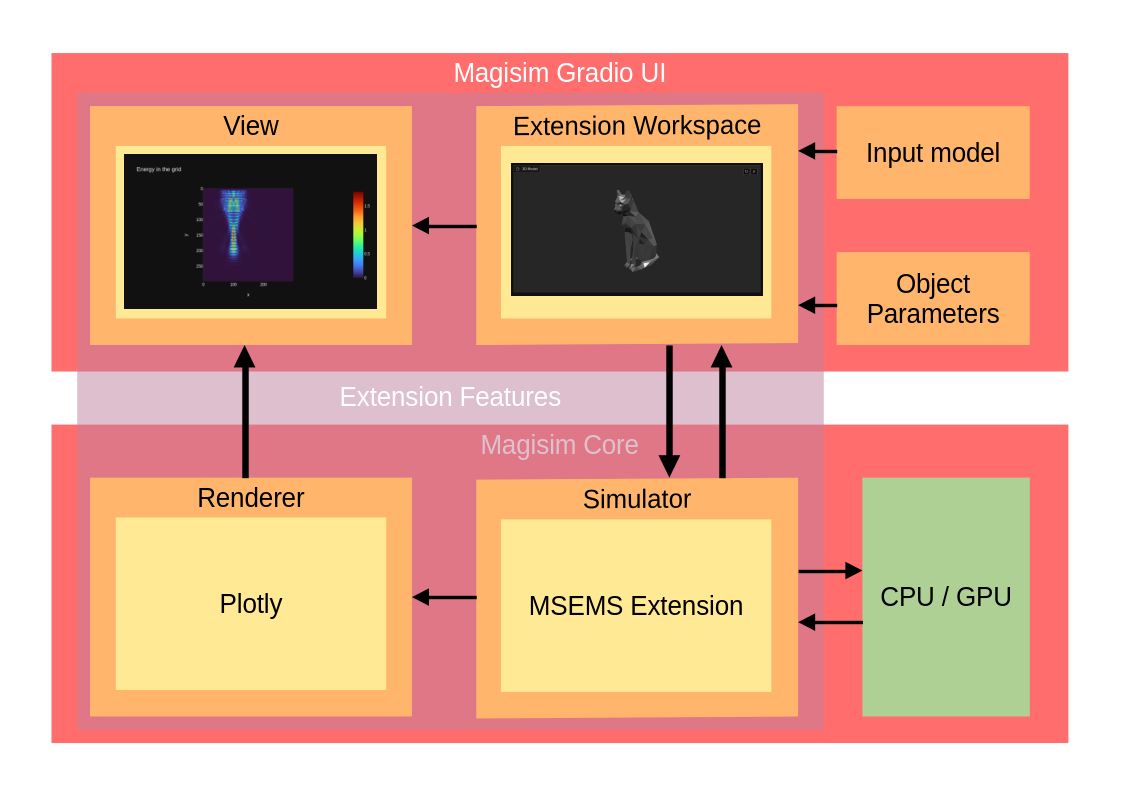
\includegraphics[width=0.8\textwidth]{softstruct.png}
\end{center}

Each extension describes its own user interface by using modules available in the Gradio package. This allows third parties to rapidly develop intuitive and efficient interfaces that integrate seamlessly with the core functionalities of Magisim. The use of Gradio's modules offers developers the flexibility to customize and extend the interface according to specific needs, promoting a high degree of adaptability and user-centric design.
\newpage
\subsubsection{Extension Model and Templates}

Aiming for high modularity, the project was structured so that every component was defined as an "Extension". This approach enabled the development of a unified system where all components adhered to a set of predefined rules, including a universal code structure. Such standardization allowed for the components to be loaded by a single function at startup, simplifying the development process and reducing program complexity.

\begin{minted}{python}
	# shared extension imports
	import gradio as gr
	from shared.builtin import Extension
	from shared.config import Config
	
	class ExtensionMeta:
	name: str = "name"
	uuid: str = "some-uuid-v4"
	authors: list = ["author"]
	version: str = "1.0.0"
	license: str = "license"
	description: str = """multiline description if needed"""

	class ExtensionType:
	types: list = [Extension.Simulator, Extension.Workspace]
	hasNodes: [(Extension,(list,list))] = [
	(Extension.Simulator, # define a simulator node
		(
			[ # inputs
				("some-input","some-type")
			],
			[ # outputs
				("some-output1","some-type"), 
				("some-output2","some-type")
			]
		)
	)]
	
	def load_workspace(app: gr.Blocks):
		with gr.Tab(ExtensionMeta.name, id=ExtensionMeta.uuid):
			gr.Markdown(ExtensionMeta.description)
			# Extension UI code

\end{minted}
\newpage

\subsubsection{Message Queue and Routing}

In defining component interaction and data handling, the initial consideration was to develop an in-house asynchronous communication layer. However, it was soon recognized that many solutions existed for such functionality. A message queue system in combination with a "Router" was chosen to enhance modularity.

\begin{center}
	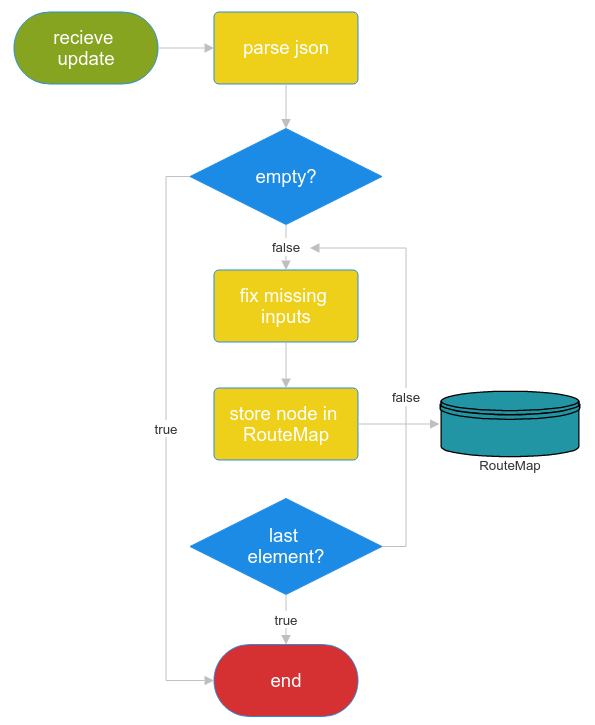
\includegraphics[width=0.8\textwidth]{nodegen-flow.png}
\end{center}

The router maps connections between extensions in a Redis database, allowing extensions to remain unaware of the destinations for their outputs. Using Python's Pickle library, the system enables the transmission of diverse data types, including 3D models and tensor arrays.






\newpage

\subsection{Scope}


\iffalse
\section{Theory}
\subsection{Maxwell's Equations}

Maxwell's equations are a fundamental set of equations in the field of electromagnetism, providing the mathematical framework for understanding the behavior of electric and magnetic fields in space and time.

Maxwell's equations consist of four essential equations that relate electric and magnetic fields to their sources (charges and currents). These equations can be expressed as follows:
\begin{center}
	1. \textbf{Gauss's Law for Electricity (Coulomb's Law):}
	
	\[
	\nabla \cdot \mathbf{E} = \frac{\rho}{\varepsilon_0}
	\]
	
	Here, \(\nabla \cdot \mathbf{E}\) represents the divergence of the electric field, and \(\varepsilon_0\) is the permittivity of free space.
\end{center}
\begin{center}
	2. \textbf{Gauss's Law for Magnetism:}
	
	\[
	\nabla \cdot \mathbf{B} = 0
	\]
	
	This equation states that magnetic field lines are always closed loops and that there are no magnetic monopoles.
\end{center}
\begin{center}
	3. \textbf{Faraday's Law of Electromagnetic Induction:}
	
	\[
	\nabla \times \mathbf{E} = -\frac{\partial \mathbf{B}}{\partial t}
	\]
	
	It describes how a changing magnetic field induces an electromotive force (EMF).
\end{center}
\begin{center}
	4. \textbf{Ampère's Circuital Law with Maxwell's Addition:}
	
	\[
	\nabla \times \mathbf{B} = \mu_0 \mathbf{J} + \mu_0 \varepsilon_0 \frac{\partial \mathbf{E}}{\partial t}
	\]
	
	This equation relates the circulation of the magnetic field (\(\oint \mathbf{B} \cdot d\mathbf{l}\)) to the electric current (\(I\)) and the rate of change of electric flux (\(\partial \mathbf{E}/\partial t\)). 
\end{center}

\newpage
\subsection{FDTD: Applying Maxwell's Equations in the Time Domain}

The Finite-Difference Time-Domain (FDTD) method is a powerful numerical technique used to solve Maxwell's equations in the time domain. It is a fundamental approach in computational electromagnetics, allowing for the simulation of electromagnetic wave propagation, interactions with materials, and the prediction of complex electromagnetic phenomena.

\subsubsection{Overview of the FDTD Method}

The FDTD method discretizes both time and space, allowing for the direct integration of Maxwell's equations in their time-domain form. This discretization divides the simulation domain into a grid of discrete points in both space and time. At each grid point, electromagnetic field values (electric and magnetic fields) are computed iteratively, advancing in discrete time steps.

\subsubsection{Time-Stepping Scheme}

In the FDTD method, the update of electromagnetic field components at each grid point follows a time-stepping scheme. The update equations are based on the finite-difference approximations of Maxwell's equations. For example, the update equations for the electric field (\(E\)) and magnetic field (\(H\)) components in 3D space can be expressed as:

\begin{center} For the electric field: \end{center}
\[
E_x^{n+1}(i,j,k) = E_x^n(i,j,k) + \frac{\Delta t}{\varepsilon(i,j,k)} \left(\nabla \times H\right)_x^n(i,j,k)
\]
\begin{center}and similarly for  $E_y$ and $E_z$\end{center}



\begin{center}For the magnetic field:\end{center}
\[
H_x^{n+1}(i,j,k) = H_x^n(i,j,k) + \frac{\Delta t}{\mu(i,j,k)} \left(\nabla \times E\right)_x^n(i,j,k)
\]
 \begin{center}and similarly for $H_y$ and $H_z$\end{center}
 
 
Here, \(n\) represents the time step, \(\Delta t\) is the time step size, and \(\varepsilon\) and \(\mu\) are the permittivity and permeability of the material at the grid point (\(i, j, k\)).
\newpage
\subsubsection{Significance in Magnetic Field Simulations}
The FDTD method is particularly significant in magnetic field simulations due to its ability to capture complex temporal behaviors of electromagnetic phenomena. It allows researchers and engineers to study magnetic field interactions with materials, structures, and devices over time. This is crucial in applications such as:
\begin{itemize}
	\item Magnetic resonance imaging (MRI)
	\item Magnetic shielding design
	\item Electromagnetic compatibility (EMC) analysis
	\item Magnetic field exposure assessment
	\item Magnetic field sensor development
\end{itemize}
By directly applying Maxwell's equations in the time domain, the FDTD method provides a comprehensive understanding of the dynamic behavior of magnetic fields, making it an indispensable tool in computational electromagnetics. 
\subsection{The compromise between accuracy and speed}
Achieving high simulation accuracy is every developers goal, especially in scientific research and mission-critical engineering applications. Accurate simulations yield results that closely mirror real-world phenomena, enabling scientists and engineers to make informed decisions, validate theoretical models, and gain deeper insights into the behavior of magnetic fields. 
Conversely, computational speed is of equal importance, particularly when dealing with large-scale simulations or real-time applications. In today's fast-paced technological landscape, there's a growing demand for swift results. Delays caused by sluggish simulations can hinder progress and decrease the end users engagement with the product. 

\newpage

\subsection{Computation}
\subsubsection{Introduction to parallel computing}
A regular computer usually performs tasks serially, one operation at a time. While this might be the most efficient method for everyday tasks, it does not apply to computationally heavy tasks spanning multiple dimensions or matrix operations. This has largely been solved today thanks to the GPU (Graphics Processing Unit) or graphics card as it is more commonly referred to as.
\subsubsection{The application of parallel computation in time domain field simulations}
Computation is a critical aspect of time domain field simulations. These simulations involve solving complex differential mathematical models and processing large datasets, which can be extremely computationally demanding. The traditional serial computing approach is therefore insufficient for handling the computational complexity associated with magnetic field simulations.

To address these challenges, we turn to parallelization, a technique that enables concurrent execution of computations across multiple processors or cores. Modern GPUs, designed for parallel processing, have become instrumental in accelerating computational tasks, including solving differential equations such as Maxwell's equations.


%According to Moore's Law, the amount of transistors in a given area of microchips are doubled every year. 


%With parallelization, the effectiveness of a computational can be increased drastically, essentially allowing for $n-1$ dimensional computation as illustrated in the below visualizations.
\fi
\newpage
\section{Approach}

\subsection{Software Structure}




\subsection{User Interface}

The UI (User Interface) for Magisim is built using Gradio, a toolkit originally developed for rapid development of interfaces for Machine Learning projects. We found this 


\subsection{Application Backbone}




\subsection{Our FDTD Extension}
In the development of our simulator extension, we initially planned to create a custom framework for Finite-Difference Time-Domain (FDTD) simulations. However, it soon became clear that developing our own framework from scratch was both impractical and unnecessary, considering the variety of existing FDTD libraries available in Python.

We built our FDTD-simulation extension upon the library developed by Floris Laporte, which provides a robust framework for conducting Finite-Difference Time-Domain (FDTD) simulations.

\subsection{Software Distribution}


\newpage
\section{Result}
\newpage
\section{Discussion}
\newpage
\section{Conclusion}
\newpage
\section{References}
Liebig, T., Rennings, A., Held, S., \& Erni, D. (2012). openEMS – a free and open source equivalent‐circuit (EC) FDTD simulation platform supporting cylindrical coordinates suitable for the analysis of traveling wave MRI applications. International Journal of Numerical Modelling (Print), 26(6), 680–696. https://doi.org/10.1002/jnm.1875

Laporte, Floris. (2020). Novel architectures for brain-inspired photonic computers [PhD Thesis]. Ghent University.

Kozlov, M., \& Turner, R. (2010). A Comparison of Ansoft HFSS and CST Microwave Studio Simulation Software for Multi-channel Coil Design and SAR Estimation at 7 T MRI. PIERS ONLINE, 6(4), 395.



\newpage
\newpage
\addcontentsline{toc}{section}{References} 
\printbibliography




\begin{center}
	\large\textbf{Written in \LaTeX}
\end{center}

\end{document}          
